\chapter{System Architecture}
\label{chp:architecture}
\section{Taxonomy}
\label{sec:taxonomy}
We define a taxonomy for observations and explanations. This taxonomy will help us standardize different approaches to explanation. It will also help us compare these approaches against each other. Our observation/explanation standard is based on the assumption that observations take the form of a query, whereas, explanations take the form of a predicate. Let $D$ be the dataset that we are interested in. Let $A_D$ be a set of attributes of $D$. Let $V_a$ represent the set of values for in $D$ for attribute $a$ where $\{\neg \emptyset,\emptyset\} \subset V_a$. Then we can define our candidate explanation $\phi$ as $$\phi \models \wedge_{i,j} {(i=j)}$$ where $i \in A_D, j \in V_i $

The observation is simply just any aggregate query on $D$. Each approach returns a set of candidate explanation and a value which scores the candidate explanation. The candidate explanations with the best scores is the best explanation.

\subsection{Non spatial explanation for non spatial observations}
\label{sec:nonspatial_nonspatial}

Non spatial observations are aggregate queries on $D$. These queries can take any form. Non spatial explanations are candidate explanations based purely on non spatial attributes of the data. Let $S$ be the spatial attributes in $D$. Our candidate explanation can be defined as 
$$\phi \models \wedge_{i,j} {(i=j)}$$
where $i \in A_D, i \notin S, j \in V_i$

We can look at an example of non spatial explanations for non spatial observations by looking at the NYC TLC data for Yellow Cab. If we consider all of the possible permutations of attributes and values in the data, it well exceeds a million permutations. Instead each of the approach we discuss tries to simplify how the explanations are calculated. For instance, salient features uses data that stands out for its explanations. Fig.~\ref{fig:yellowstats} shows the average number of taxi trips per day for one month. If we consider twenty thousand trips as an upper bound, we only get part of the curve which we call a salient feature(Section~\ref{sec:salient_features}). We can use this salient feature for our explanations. 


\subsection{Spatial explanations for non spatial observations}
\label{sec:spatial_nonspatial}

Spatial explanations take the spatial attributes of the data into consideration. In contrast to non spatial explanations, the candidate explanations for spatial explanations contain polygons. Let $S$ be the spatial attributes of $D$. Let $P$ be the set of all possible polygons from $S$. Let $G$ be a function such that$G(s,t)$ is true when $(s,t) \in P$ and false otherwise, where s,t are the dimensions of a point in the Cartesian plane. Our candidate explanation can be defined as,
$$\phi  \models \vee_{l,k} G(l,k)$$
where $k,l \in A_D$

To illustrate spatial explanation in action, we can use NYC TLC data again. Fig.~\ref{fig:spatial_explanation_example} shows the explanation in terms of tip percentage where the observation is also average tip percentage. 

\begin{figure}[ht]
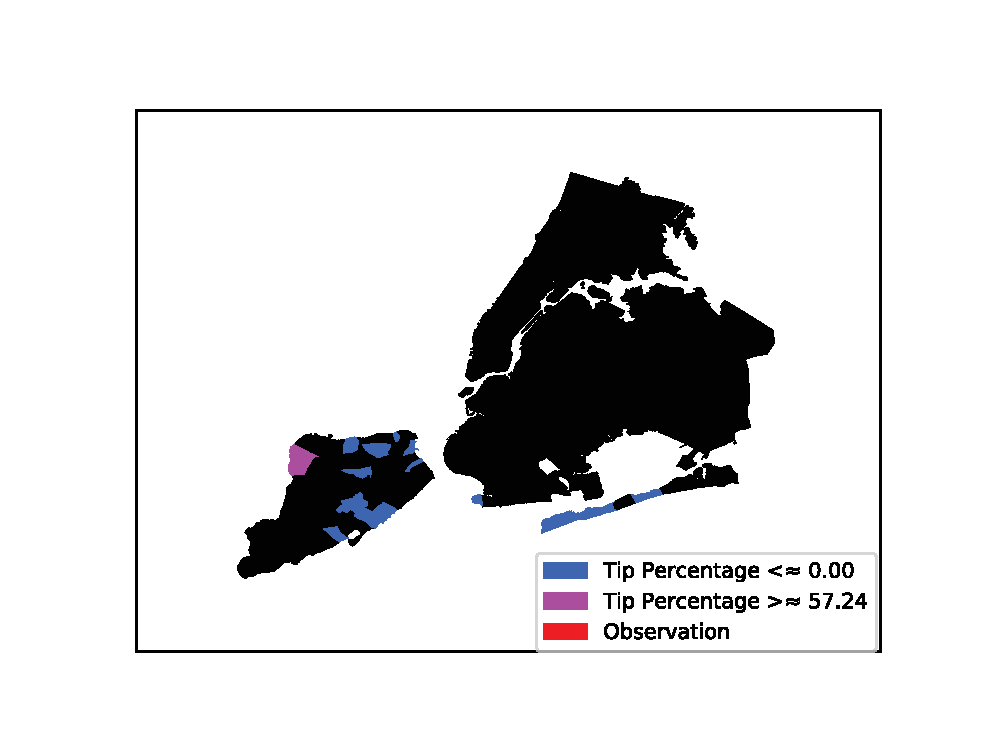
\includegraphics[width=\columnwidth]{spatial_explanation_example.eps}
\caption{An example of spatial explanation}
\label{fig:spatial_explanation_example}
\end{figure}

The polygons painted purple show polygons in the candidate explanation where tip percentage is high, while polygons painted blue show candidate explanations where tip percentage is low. It should be noted that $P$ has a high number of permutations. It is up to the approach to decide which polygons to include in the candidate explanation. For instance, hierarchical intervention may choose polygons in a spatial proximity while aggravation may choose otherwise.
\begin{figure}[ht]
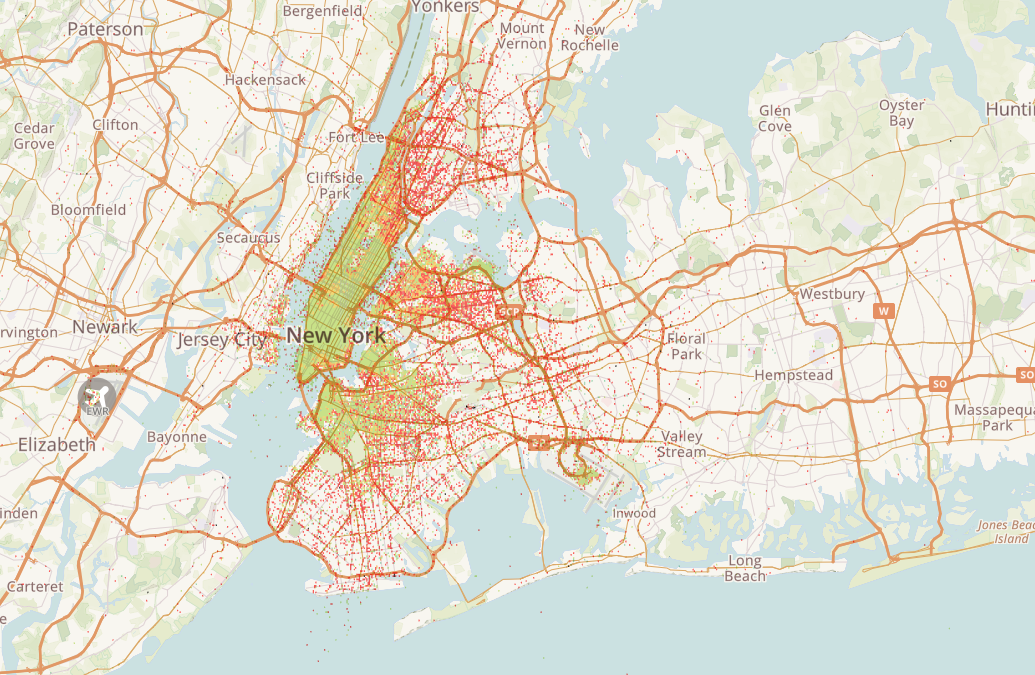
\includegraphics[width=\columnwidth]{scatter.png}
\caption{Heatmap for NYC trips for January 2016}
\label{fig:square_unit_grid}
\end{figure}

Another interesting consideration when we are talking about spatial explanations is the density of the data. Fig.~\ref{fig:square_unit_grid} shows the square unit cartogram for tip percentage in with respect to pickup coordinates. It is interesting to observe that the explanations provided in Fig.~\ref{fig:spatial_explanation_example} are all areas with low density of data. One of the reasons for this is because each approach takes some liberty with our definition of the taxonomy. Eventhough, we defined $P$ to contain all permutations of polygons. An approach may use limited polygons, such as neighborhoods or zones. The way the the explanation is ranked also plays a large role.

\subsection{Spatial explanations for spatial observations}
\label{sec:spatial_spatial}
In the last two classes of our taxonomy, we only looked at non spatial observations. In this class however, we will look at spatial observations. Spatial observations are similar to non spatial observation. Both spatial and non spatial observations are represented by an aggregate query. The difference is that spatial observations have a polygon in the predicate. The spatial explanation in this class can be defined in the same way as in Section~\ref{sec:spatial_nonspatial}. 

\begin{wrapfigure}{r}{0.5\textwidth}
  \begin{center}
    \includegraphics[width=0.48\textwidth]{spatial_spatial_vertical.eps}
  \end{center}
  \caption{An example of spatial explanation for a spatial observation}
\label{fig:spatial_spatial_vertical}
\end{wrapfigure}



Fig.~\ref{fig:spatial_spatial_vertical} shows an example of a spatial explanation for a spatial observation. The observation in this case is the average tip percentage when the pickup zone is LaGuardia airport. The candidate explanation displayed are also based on tip percentage, though they could have been any other attribute as well. Introducing a spatial predicate has a large observable impact on the explanation compared to the one in Section~\ref{sec:spatial_nonspatial}


\section{Studied Approaches}
\label{sec:approaches}
There are three main approaches that we use in this thesis. Aggravation, Intervention and Salient Features. We also introduce hierarchical intervention. This approach is an extension of intervention which takes spatial clusters into account. Originally, Aggravation and Intervention were used in a non spatial context in related works\citep{chirigati2016data}. However, we extended these solutions to fit into our spatial taxonomy. 

\subsection{Aggravation}
\label{sec:aggravation}

The first approach we will look at for explanation is aggravation. This approach tries to look at tuples which 'aggravate' the results. The main idea is to calculate the value of the observation for each candidate explanation. The candidate explanation with the highest value has the highest weight as the explanation. 

Let $q$ be our observation query(aggregate query). Let $\phi$ be our candidate explanation. Let $D_\phi$ be the dataset that satisfies our candidate explanation i.e. $D_\phi = \sigma_\phi(D)$. Let $Q$ be a scalar function that takes in a dataset and gives the value obtained when $q$ is applied on this data. The degree of candidate explanation, $\delta_{agg}$, by aggravation can be simplified as $Q(D_\phi)$. 

In order to have a degree of explanation which is high when we are closer to our desired explanation, we need to have a direction for our explanation. For example, if we want to observe high values of tip percentage in the NYC TLC data, our direction will be high. If we want to observe lower values of tip percentage, our direction will be low. If our direction is low, we are interested in the lower values. However since we want our degree of candidate explanation to be higher when we have the desired candidate explanation, we can simply reassign its value.

\begin{equation}
\delta_{agg}:=
    \begin{cases}
      Q(D_\phi), & \text{if}\ direction=high \\
      -Q(\phi), & \text{otherwise}
    \end{cases}
\end{equation}

% Bucketing values
In order to decrease the number of permutations for candidate explanations, we can bucket the values. Consider an attribute $a$ in the dataset. Let $V_a$ represent each value that $a$ can takes up, where $V_a=\{v_1,v_2,...,v_n\}$ and $n$ is the number of tuples. Let the minimum value in $V_a$ be represented by $a_{min}$.The mean value, $\mu$, is defined as $\frac{\Sigma_iv_i}{n}$. The standard deviation, $\sigma$, is defined as $\sqrt{\frac{1}{n-1}\Sigma_i(v_i-\mu)^2}$. Each value is assigned to a bucket. Let $b_i$ be the bucket the value, $v_i$ is assigned to. Then $$b_i = \bigg \lfloor\frac{v_i-a_{min}}{\sigma} \bigg \rfloor$$

Now, instead of using all the permutations in $V_a$ as part of our candidate explanations, we can rather use all the distinct values of buckets. The predicate represented by each bucket $b_i$ is simply
$$ a \geq (a_{min}+b_i\times\sigma) \wedge a < (a_{min}+b_i\times(\sigma+1))$$
This decreases the number of permutions for candidate explanations by a factor of $\frac{1}{\sigma}$

\renewcommand{\lstlistingname}{Query}% Listing -> Algorithm
\begin{lstlisting}[language=SQL, caption=Aggregate Query for average tip percentage, label=qry:aggregate]
SELECT AVG(trip_distance) FROM
FROM nyc_data
\end{lstlisting}

As an hands on example of this approach consider the observation on the NYC TLC data represented in Query~\ref{qry:aggregate}. We are interested in the candidate explanation in the context of the number of passengers. The top explanation for this observation gives $Q=6.00$, $b_i=3$. Since we know the bucket and $\sigma$. The explanation predicate turns out to be $passenger\_count \geq 3.97 \wedge passenger\_count < 5.30$. If you are a yellow cab driver, this explanation may tell you to be prepared for a long trip if you have four or five passengers.

Now that we have described the aggravation approach for the nonspatial case, we can extend it to handle spatial observations and expanations. We introduce a dataset of polygons $P$. The set $P$ consists of distinct non overlapping polygons over our dataset $D$. Let $s$,$t$ be the spatial attributes in $D$. Each tuple in $P$ has two attributes: $polygon\_id$, and $polygon$. We create a new dataset 
$$D' \leftarrow D \bowtie_{contains(P.polygon,(s,t))} P$$

Now we can use our spatial candidate explanations and observations defined in our taxonomy(Section~\ref{sec:taxonomy}) on out new dataset $D'$

\subsection{Intervention}
\label{sec:intervention}

Intervention is an approach inspired by the concept of influence. It builds on the aggravation approach(Section~\ref{sec:aggravation}). Intervention tries to measure how much our observations would change had our explanation not be present. Let $D$ be the dataset we are interested in. Let $Q$ be a function which returns the value of our observation given a dataset. Keeping our taxonomy in context, this means $Q$ returns the value of our aggregate observation query. Let $\phi$ be our candidate explanation. Let $\Delta_\phi \leftarrow \sigma_\phi(D)$. Let $D_\phi = D - \Delta_\phi$. The direction of our observation can either be \textit{high} or \textit{low} depending on whether we are interested in the greatest or least values of observation respectively. Our degree of candidate explanation by intervention, $\delta_{int}$, can then be expressed as,
\begin{equation}
\delta_{int}:=
    \begin{cases}
        -Q(D_\phi), & \text{if}\ direction=high \\
        Q(D_\phi), & \text{otherwise}
    \end{cases}
\end{equation}

We want the degree of candidate explanation by intervention to be higher, the closer we are to the direction of the observation, therefore, we use the negative value when the direction is high. If the influence of the candidate explanation is high, it will result in a low observation value once the candidate explanation is removed from the dataset.

Since intervention extends the idea presented by aggravation, it has similar issues when it comes to the number of permutations for candidate explanations. Similar to our approach in aggravation(Section~\ref{sec:aggravation}), we can reduce the number of permutations by bucketing the attributes. We can extend intervention for spatial observations and explanations, the same way we did for aggravation. The set $P$ consists of distinct non overlapping polygons over our dataset $D$. Let $s$,$t$ be the spatial attributes in $D$. Each tuple in $P$ has two attributes: $polygon\_id$, and $polygon$. We create a new dataset 
$D' \leftarrow D \bowtie_{contains(P.polygon,(s,t))} P$. Spatial observations can now be defined as aggregate queries with a predicate containing $P.polygon$. Candidate spatial explanations can be defined as candidate explanations containing $P.polygon$ as emphasized in our taxonomy(Section~\ref{sec:taxonomy}). 

\begin{figure}[ht]
\begin{center}
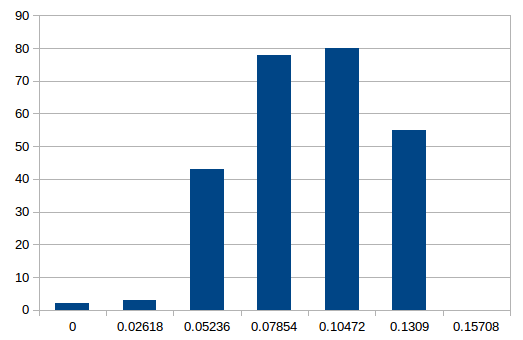
\includegraphics[width=0.5\columnwidth]{spatial_aggravation_histogram.png}
\end{center}
\caption{Number of Zones against Degree of Spatial Aggravation}
\label{fig:spatial_aggravation_histogram}
\end{figure}

\begin{figure}[ht]
\begin{center}
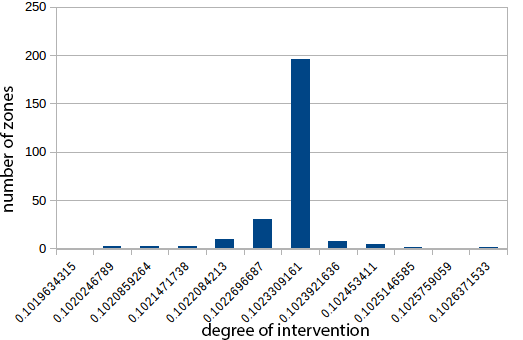
\includegraphics[width=0.5\columnwidth]{spatial_intervention_histogram.png}
\end{center}
\caption{Number of zones against their degree of Spatial Intervention}
\label{fig:spatial_intervention_histogram}
\end{figure}

In order to compare the differences between aggravation and intervention, it is helpful to look at their degrees of aggravation and intervention respectively. As an example, we look at the NYC TLC data where $P$ is the set of taxi zones. Fig.~\ref{fig:spatial_aggravation_histogram} shows a histogram for the number of taxi zones which fall inside different range of the degree of candidate explanation by aggravation. Fig.~\ref{fig:spatial_intervention_histogram} shows a similar histogram for the number of zones which between certain ranges for the degree of candidate explanation by intervention. The observation in both cases is the average tip percentage. It is immediately evident from these two histograms that the domain for explanation by aggravation is 150 times larger than intervention while the range for explanation by intervention is 2.5 times larger than aggravation in this instance of the problem. The reason for having a small domain for intervention is because the influence of removing one of the zones on the observation is very small, whereas, each zone may have a large difference in average tip percentage compared to other zones. We will look further into the implications of these differences when we evaluate(Section~\ref{sec:evaluation}) these approaches.

\subsection{Salient Features}
\label{sec:salient_features}

Another approach for finding explanations is the use of salient features. As the name suggests, salient features intend to highlight portions of data which stand out. One of the examples which illustrates this can be seen in Fig.~\ref{fig:yellowstats}. The figure shows the average number of taxi trips per day over the course of a month. There is a large noticeable decline in the number of trips. The data representing this decline can be considered as a salient feature. Salient features like these tell a lot about the data. For example, if you were to look up the date illustrated in the example where the number of taxi trips drop, you would find that there was a travel ban because of extreme weather conditions. 

Salient features are based on temporal or spatio temporal scalar functions. We define two types of scalar functions: 1-D scalar functions and 2-D scalar functions. 1-D scalar functions map time to a scalar value. For example, the data presented in Fig.~\ref{fig:yellowstats} maps time to the number of taxi trips. 2-D scalar functions map time and space to a scalar value.  Fig.~\ref{fig:spatial_explanation_example} shows an example of a 2-D scalar function for one time step. Since our taxonomy is concerned with only the spatial domain of this problem. We will be considering a 2-D scalar function where one time step covers the entire scope of our dataset i.e. 1-D scalar function based on space. 

Now that we understand what salient features are, the natural question would be how to find salient features in a dataset. In order to calculate salient features, we define two threshold values $\theta^+$ and $\theta^-$. \textit{Positive salient features} are the parts of our scalar function where its value is greater than $\theta^+$ i.e. $f^{-1}([\theta^+, \infty))$. \textit{Negative salient features} are the parts of our scalar function where its value is less than $\theta^-$ i.e. $f^{-1}((-\infty, \theta^-])$. The local maxima and minima are referred to as \textit{critical points} i.e. $\nabla f = 0$

Our extension of this approach for spatial explanation stems from the fact that each feature can be represented as a predicate. For instance if we consider the function represented in Fig.~\ref{fig:yellowstats}. Let $\theta^-$ be 20,000. Then the negative salient feature can be represented as a predicate based on time and the number of trips. In the case of a 2-D scalar function, the predicate would be based on the time, attribute, and a polygon. In case of a 1-D spatial scalar function, the predicate would consist of a polygon, and an attribute. In order to calculate an explanation, we measure the co relation between scalar functions of different attributes in a dataset. Let $f_1$ be the scalar function for one attribute and $f_2$ be the scalar function of another attribute. Let $F_1$ and $F_2$ be the features of $f_1$ and $f_2$ respectively. We define $F = F_1 \cap F_2$ be the set of features both $f_1$ and $f_2$ have in common. $f_1$ and $f_2$ are \textit{feature related} at a point $x$ if $x \in F$, where $x$ has spatial and/or temporal dimensions depending on our scalar functions. $f_1$ and $f_2$ can be positively or negatively related. Let $F^+ = F_1^+ \cap F_2^+$ where $F_1^+$ and $F_2^+$ are positive features of $f_1$ and $f_2$ respectively. Let $F^- = F_1^- \cap F_2^-$ where $F_1^-$ and $F_2^-$ are negative features of $f_1$ and $f_2$ respectively. Then $f_1$ and $f_2$ are positively related at $x$ if $x \in F^+$  or $x \in F^-$. $f_1$ and $f_2$ are negatively related at $x$ if $x \notin F^+\ \text{and}\ x \notin F^-\ \text{and}\ x\in F$. 

The value of relation ship score, $\tau$, can help us decide whether two attributes are co related. If the attributes are related, then their features can be represented as candidate explanations. Let $p$ be the set of positive relations in $F$. Let $n$ be the set of negative relations in $F$. Then,
$\tau = \frac{|p|-|n|}{|F|}$


Our system uses the salient features implementation by F. Chirigati et. al in their work on Data Polygamy framework. Calculating salient features consists of three main steps: Pre processing, aggregation, and indexing. Each step in this process is implemented as a map reduce operation. 

In the preprocessing step, the spatial and temporal attributes of the dataset are used to select the data. The spatial and temporal attributes form the key in the mapreduce job while the average of our attributes form the value. In the aggregation step, the scalar functions are generated for the data. Each attribute in our dataset is represented by a different scalar function. Several scalar functions are calculated for each attribute for each spatio temporal resolution e.g. the spatio temporal resolution of hour and neighborhood has a different scalar function than the scalar function for day and zipcode. The next step consists of indexing the data. Indexing consists of creating a graph out of the aggregated data. Each node in the graph represents a point in the spatiotemporal domain. It may be convenient to think of this as a 2-D graph where one axis represents space and another represents time. A node is connected to another node if they are adjacent to each other in space(e.g. two neighborhoods next to each other) and time. The value if each node is the average attribute value. Due to the nature of the data, some points in the graph might be missing. The indexing step linearly interpolates the missing points in the graph. The 2-D scalar functions we calculated are finally used to calculate whether each node in our graph is a negative salient feature or positive salient feature.

After the salient features are calculated we need to measure how well they explain the data. We do this by finding the relationship score between the observation scalar function and the scalar function for the remaining attributes in our dataset. The non spatial explanation consists of our threshold values while the spatial explanation consists of the polygons represented by the co-related salient features.